% arara: xelatex: { shell: yes }
% arara: bibtex
% arara: xelatex: { shell: yes }
% arara: xelatex: { shell: yes }


% options:
% thesis=B bachelor's thesis
% thesis=M master's thesis
% czech thesis in Czech language
% english thesis in English language
% hidelinks remove colour boxes around hyperlinks

\documentclass[thesis=M,english]{FITthesis}[2019/12/23]

%\usepackage[utf8]{inputenc} % LaTeX source encoded as UTF-8
% \usepackage[latin2]{inputenc} % LaTeX source encoded as ISO-8859-2
% \usepackage[cp1250]{inputenc} % LaTeX source encoded as Windows-1250

% \usepackage{subfig} %subfigures
% \usepackage{amsmath} %advanced maths
% \usepackage{amssymb} %additional math symbols

\usepackage{dirtree} %directory tree visualisation
\usepackage{minted}
\usepackage{xcolor}
\usepackage{array}

% list padding
\usepackage{enumitem}

\definecolor{LightGray}{gray}{0.9}

% % list of acronyms
% \usepackage[acronym,nonumberlist,toc,numberedsection=autolabel]{glossaries}
% \iflanguage{czech}{\renewcommand*{\acronymname}{Seznam pou{\v z}it{\' y}ch zkratek}}{}
% \makeglossaries

% % % % % % % % % % % % % % % % % % % % % % % % % % % % % %
% EDIT THIS
% % % % % % % % % % % % % % % % % % % % % % % % % % % % % %

\department{Department of software engineering}
\title{Neo4j .NET ORM}
\authorGN{} %author's given name/names
\authorFN{Starý} %author's surname
\author{Tomáš} %author's name without academic degrees
\authorWithDegrees{Bc. Tomáš Starý} %author's name with academic degrees
\supervisor{Ing. Marek Skotnica}
\acknowledgements{THANKS (remove entirely in case you do not with to thank anyone)}
\abstractEN{Summarize the contents and contribution of your work in a few sentences in English language.}
\abstractCS{V n{\v e}kolika v{\v e}t{\' a}ch shr{\v n}te obsah a p{\v r}{\' i}nos t{\' e}to pr{\' a}ce v {\v c}esk{\' e}m jazyce.}
\placeForDeclarationOfAuthenticity{Prague}
\keywordsCS{Replace with comma-separated list of keywords in Czech.}
\keywordsEN{Replace with comma-separated list of keywords in English.}
\declarationOfAuthenticityOption{1} %select as appropriate, according to the desired license (integer 1-6)
% \website{http://site.example/thesis} %optional thesis URL


\begin{document}

% \newacronym{CVUT}{{\v C}VUT}{{\v C}esk{\' e} vysok{\' e} u{\v c}en{\' i} technick{\' e} v Praze}
% \newacronym{FIT}{FIT}{Fakulta informa{\v c}n{\' i}ch technologi{\' i}}

% \setsecnumdepth{part}

\begin{introduction}

    \section{Graphs are everywhere}

    In today's world, everything is highly connected.
    Graphs are an easy way to describe and visualize these relations and can help to see connections we would not otherwise catch.

    We do not use graphs to store data in most of our applications today, mainly because the first applications were made to take paper forms into the digital world.
    To keep these paper forms in digital format, we use relational databases.

    Since then, relational databases have been the go-to for every developer when creating a new application.
    Using a relational database is helpful for several reasons, mainly because the development cost is lower than using new technologies, and everyone is familiar with this type of \acrshort{dbms}.
    However, the lower development price benefits are diminished in today's world by the numerous problems with using relational databases.
    For example, lengthy searches for specific highly connected data and more complex relations are the main reason why \Gls{nosql} databases have been gaining so many tractions for the last decade.

    The graph databases are made explicitly with relationships in mind.
    Every vertex can have its connection with another one or even itself.
    This kind of connection is not possible with a relational database where connecting two rows means creating a relationship between two tables.
    To help with the performance of finding highly connected data, users can define indexes in relational databases, but there is only so much he can do.
    Indexes can slow the whole system down, inserts will be longer, and the entire database will increase memory consumption.

    \subsection{What can graph databases offer?}

    Graph databases are no silver bullet, and they cannot solve all our problems.
    When designing a new piece of software, we should always ask ourselves what the best technologies for the situation we are trying to solve is.

    We have discussed the problem with highly connected data and long searches, but how does the graph database solve this issue?
    The key here is that we will sooner or later find out that with more data comes more time spent on the same select with a growing relational database.
    This behaviour is due to numerous reasons, but the main one is that we are bound to make more costly joins with more extensive tables.
    Our search will be over the same part of the graph with a graph database no matter what happens with the rest. Execution times should therefore be the same.

    \section{How to use graph databases with object-oriented languages?}

    In most applications that communicate with a database, developers use an \acrshort{orm} to create objects from the database.
    This is a widespread way to use databases, and it is effortless to use. It creates an abstraction between the object-oriented language and \acrshort{sql}.
    Thus developers do not need a deep knowledge of \acrshort{sql} to use it.

    \acrshort{orm}s are powerful, but they are used only with relational databases, which is understandable given that \acrshort{orm} stands for Object-Relational Mapper.
    If we would like to use a mapper between a graph database and an object-oriented language, we would call it an \acrfull{ogm}. These types of mappers are not as widespread as \acrshort{orm}s are.

    In this paper, we will go through the steps of creating the \acrshort{ogm} library for \CS.
    We will start by studying graph databases and their query languages, studying similar solutions, namely EntityFramework, and end with our design and implementation of the library with proper testing.

\end{introduction}


\chapter {Analysis}

\section {Graph databases}

Graph databases store information in graphs, very similarly as relation databases store information in tables and have relations between columns in tables, graph databases store information in nodes and even on the edges, or as we should call them, relations.

In contrast to most relational databases, graph databases are schemaless, meaning that they do not have described schema of each node.

Let us show the power of graph databases in a real-world example. Social networks dominate today's internet content, and everyone wants to be connected with his or her friends and relatives. In one of the social networks, we have people who can post their thoughts or opinions.
Other users can follow them to see their posts, and also they can like those posts. We can identify two entities with relations between them. In a relational database, it would look like this.

\begin{figure}[H]
    \centering
    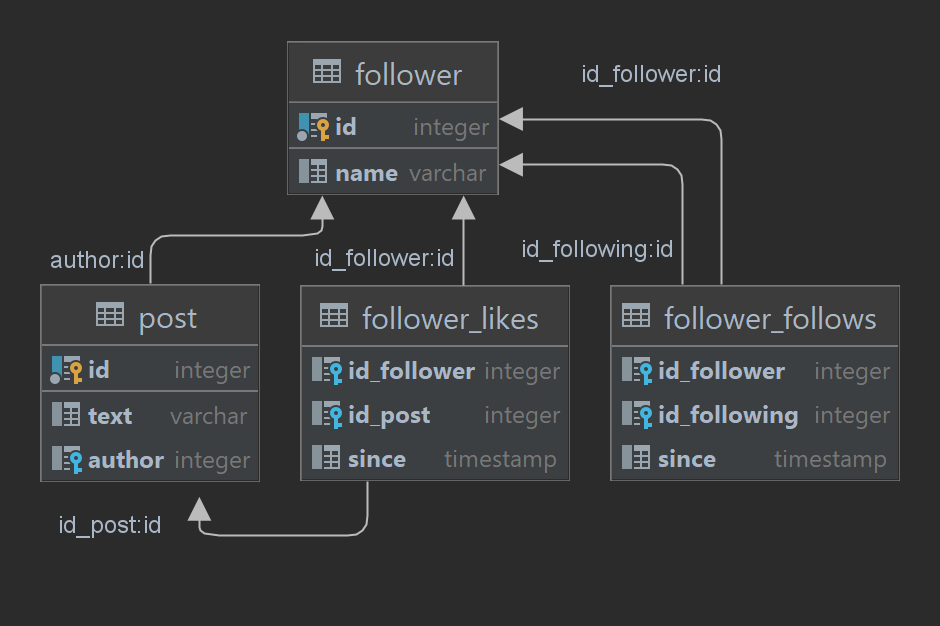
\includegraphics[width=0.8\textwidth]{content/relational-dbms-social-network.png}
\end{figure}

We need four tables and five foreign keys to describe all relations between two identified entities. This can lead to costly joins to answer requests resulting from relationships between entities. For example, we could ask who follows followers who liked someone's post. The query for this example could then look like this:

\begin{listing}[H]
    \begin{minted}
    [
    frame=lines,
    framesep=2mm,
    baselinestretch=1.2,
    bgcolor=LightGray,
    linenos,
    breaklines
    ] {sql}
SELECT followers_of_followers_data.*
FROM post
JOIN follower_likes fl ON post.id = fl.id_post
JOIN follower followers_liked ON fl.id_follower = followers_liked.id
JOIN follower_follows followers_of_followers ON followers_liked.id = followers_of_followers.id_following
JOIN follower followers_of_followers_data ON followers_of_followers.id_follower = followers_of_followers_data.id
WHERE post.id = :post_id
ORDER BY followers_of_followers_data.name;
    \end{minted}
\end{listing}

From the query, we can see that it is barely readable and complex. However, the main problem is performance. The join operations will take more time even for the same request, with more data stored in tables. Let us now compare the same problem solved using a graph database.

\begin{figure}[H]
    \centering
    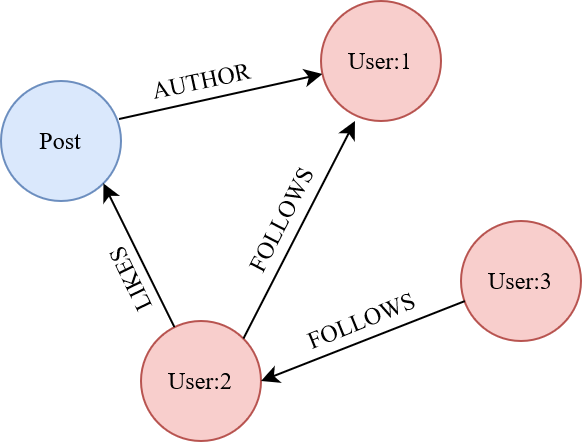
\includegraphics[width=0.8\textwidth]{content/graph_example.png}
\end{figure}

As we can see from the picture, each node has one relation or more to other nodes. Furthermore, the answer to our question from the beginning is already visible if we remind ourselves: who follows users that liked the post, we can then follow the path in the graph, and as we are going to discover in a moment, the query to get this information also follows this path.

\begin{listing}[H]
    \begin{minted}
    [
    frame=lines,
    framesep=2mm,
    baselinestretch=1.2,
    bgcolor=LightGray,
    linenos,
    breaklines
    ] {cypher}
    MATCH (:Post {id: {post_id}})-[:LIKES]->(:User)-[:FOLLOWS]->(followers:User) RETURN (followers);
    \end{minted}
\end{listing}

As promised, the query should not be hard to understand. This is just a small example of how powerful graph databases can be.

\subsection {Native vs. Non-native graph databases}

When dealing with graph databases, we have to look at two main DBMS features: storage and processing.

Storage is how graphs are stored in memory. If the storage is optimized for graphs, like having related nodes close together, then we talk about native graph storage. However, there are implementations using other NoSQL storages, called non-native graph storages.

The second feature mentioned was processing, which refers to how graph databases process database operations. What is meant by that is how the database treats queries and how it handles storage. Native databases use Index-free adjacency for processing.

\textbf{Index-free adjacency} is, in short, storing neighboring data next to each other. Now that seems too short, so in a more specific way:
"Native graphs take data that is logically connected via arcs or relationships and hard-wire the physical RAM addresses of these items into the node."
\cite{mccreary_neighborhood_2021} With this in mind, we can now see why are graph databases faster than other types of DBMS.
In traditional RDBMS, looking up a row in another table means that we have to pull an index table representing this relation and then find a path to row in said table.
In RDBMS, this leads to another problem because the database uses many indexes to keep data connected, which negatively impacts insert operations.

One more thing we should go through is how the graph database handles writes. Connected data requires strict data integrity.
Graph databases have to create or update not only nodes themselves but also relationships; otherwise, this could result in a corrupted graph, which is almost impossible to fix.
The solution to this problem is to write fully ACID-compliant transactions, ensuring that the database will not become corrupted.

\section{Neo4j}

Neo4j is a graph database management system. It is developed by Neo4j, Inc., with its origin in Sweden. Neo4j is a native graph database, and it is also ACID-compliant. Given these properties, Neo4 uses its custom query language tailored explicitly for querying over graphs, and its name is Cypher.

\subsection{More about Cypher}

Cypher is a query language used for querying over the Neo4j database. Its philosophy is to be easily read and understood by developers, database professionals, and business stakeholders. Its ease of use derives from the fact that it is in accord with how we intuitively describe graphs using diagrams. \cite{robinson_graph_2015}

\subsubsection{Match}
\subsubsection{Return}
\subsubsection{Other clauses}

\section{ORM}
ORM stands for an object-relational mapper, which is based on the concept of object-relational mapping. Object-relational mapping is the idea of writing queries using the object-oriented paradigm.
There are some limitations of what ORM can accomplish. Developers should always consider these limits before using an ORM framework. \cite{mario_hoyos_what_2018}

\noindent Pros:
\begin{itemize}
    \item There is no need to use a second language during software development, SQL is a powerful language, but most developers do not use it too often.
    \item ORM abstracts away from the database system.
    \item It can lead to better performance than writing queries by ourselves.
\end{itemize}
Cons:
\begin{itemize}
    \item If a developer is an SQL power user, he can write queries that will perform better.
    \item Developers have to learn how to use ORM properly.
    \item Developers still need to know how does ORM works under the hood.
\end{itemize}

Using the term ORM with relation to graph databases is not correct. The proper term would be OGM (object-graph mapping), but there are a few reasons why we are using ORM instead of OGM in the name of this thesis. But make no mistake, when discussing ORM involving graph databases, it is, in fact, OGM. The main reason is simple: ORM has been around for more than a decade, and developers are familiar with the concept and its challenges.

\section {Existing solutions}

\subsection {Neo4j OGM}

Neo4j company has already created an OGM for their database. It supports dynamic objects and maps nodes and their relations into the domain model. It is written in Java, but it should be a starting point when designing a similar library in the C\#.

\noindent Main features:
\begin{itemize}
    \item Object graph mapping of annotated node- and relationship-entities
    \item Neo4jSession for direct interaction with Neo4j
    \item Fast class metadata scanning
    \item Optimized management of data loading and change tracking for minimal data transfers
    \item Multiple transports: binary (bolt), HTTP and embedded
    \item Persistence lifecycle events
    \item Query result projection to DTOs
\end{itemize}

\subsubsection {Neo4j drivers}

There are three possible drivers to use, Bolt driver, HTTP driver, or embedded driver, which creates in-memory Neo4j instance.

Using a different driver in the development or test environment will not affect the production code. These drivers are interchangeable without the need for modification in queries.

\subsubsection {Entities}

This library offers us the possibility to define and shape entities and relationships. \texttt{@NodeEntity} annotation is used to declare that a POJO (Plain Old Java Object)
is indeed a node. This class must have one empty public constructor to allow the library to construct the objects.

Fields on the entity are by default mapped to properties of the node. Fields referencing other node entities (or collections thereof) are linked with relationships.

If we want to change fields name or other properties, we can use annotations like \texttt{@Property}, \texttt{@Id}, \texttt{@GeneratedValue}, or \texttt{@Relationship}. On the other hand,
if we want to not include a field in the node, we can use annotations \texttt{@Transient}.

\subsubsection {Relationships}

Every field of an entity that references one or more other node entities is backed by relationships in the graph. These relationships are managed by Neo4j-OGM automatically.

If we want to specify relationship properties, like the direction of the relationship, the \texttt{@Relationship} annotation is used. The directions are either \texttt{INCOMING},
\texttt{OUTGOING}, or \texttt{UNDIRECTED}, where the last one ensures that the path between two node entities is navigable from either side.

Neo4j gives us the ability to define properties in relationships. Neo4j solves this using an entity (POJO) with annotation \texttt{@RelationshipEntity}.

A String attribute called type is available on the @RelationshipEntity annotation to control the relationship type. Like the simple strategy for labeling node entities,
if this is not provided, then the class's name is used to derive the relationship type, although it is converted into SNAKE\_CASE to honor
the naming conventions of Neo4j relationships. \cite{noauthor_reference_nodate}

Inside the entity, we then define @StartNode and @EndNode. In referenced entities, we also define a reference to
the related entity and use @Relationship with type same as in @RelationshipEntity.

Below is an example of such usage:

\begin{listing}[!ht]
    \begin{minted}
    [
    frame=lines,
    framesep=2mm,
    baselinestretch=1.2,
    bgcolor=LightGray,
    linenos
    ] {java}
@NodeEntity
public class Actor {
    Long id;
    @Relationship(type="PLAYED_IN") private Role playedIn;
}

@RelationshipEntity(type = "PLAYED_IN")
public class Role {
    @Id @GeneratedValue   private Long relationshipId;
    @Property  private String title;
    @StartNode private Actor actor;
    @EndNode   private Movie movie;
}

@NodeEntity
public class Movie {
    private Long id;
    private String title;
}
    \end{minted}
    \caption{An example of entities with relationship as separate entity}
    \label{listing:1}
\end{listing}

\subsubsection {Indexes}

Annotations can define indexes. We already saw one of them, \texttt{@Id}, an annotation for the primary index.

But primary indexes are not the only type of index we can define in our models. We can also define indexes for other
properties using \texttt{@Index} annotation. We get an index with constraint if we use \texttt{@Index(unique=true)}.

This library also supports composite indexes and node constraints with \texttt{@CompositeIndex} and \texttt{@CompositeIndex(unique = true)}, respectively.

\texttt{@Required} is an existence constraint. "It is possible to annotate properties in both node entities and relationship entities. For node entities
the label of declaring class is used to create the constraint. For relationship entities the relationship type is used - such type must be defined on leaf class." \cite{noauthor_reference_nodate}

The OGM library can handle creating and managing indexes or constraints, but as stated in the documentation, this feature should be used only for development
and not in production. That is why this feature is, by default, turned off.


These are the available modes:
\begin{table}[H]
    \begin{center}
        \begin{tabularx}{\textwidth}{|c|p{0.83\textwidth}|}
            \hline
            node     & Default, nothing is done on the side of the OGM library.                                  \\
            \hline
            validate & This ensures that all constraints and indexes are in the database before starting up.     \\
            \hline
            assert   & This drops all indexes on startup and then creates only these defined by OGM annotations. \\
            \hline
            update   & Update indexes and constraints based on annotations.                                      \\
            \hline
            dump     & Dumps all indexes and constraints to a file.                                              \\
            \hline
        \end{tabularx}
        % TODO Caption
    \end{center}
\end{table}

\subsubsection{Sessions}
To interact with mapped entities, Neo4j-OGM requires a \texttt{Session}, which \texttt{SessionFactory} provides. Besides providing \texttt{Session}, \texttt{SessionFactory} also setups up the object graph mapping metadata when constructed. That is then used across all \texttt{Session} objects created by \texttt{SessionFactory}.

Session keeps track of mapped entities, their changes, and changes between their relationships. Tracking is then used when saving or otherwise working with mapped entities. When an entity is loaded by session, reloading this entity is then done from cache within the session.

To keep new data and not prolong sessions too much, session lifetime can be managed in code. Too long session lifetime means that other users can change data, and too short a lifetime means costly save operations will be executed more often. There is a way to force the session's cache to clear, but it is advised against it.

Cypher drives Neo4j-OGM queries only. This means that only CRUD (Create Read Update and Delete) operations are available. Documentation suggests using server-side operations for more complex or performant graph traversals over the graph. Nevertheless, Cypher should be powerful enough for most of the problems.

\subsubsection {Persisting entities}

Session allows to save, load, loadAll, and delete entities with transaction handling, and exception translation managed. Persistence is performed through method save. This method then looks at underlying MappingContext and compares data loaded from the database with the saved entity, creating appropriate Cypher queries to update the database based on differences. Calling save is necessary to propagate changes because Neo4j-OGM does not automatically commit changes.

The method has a second optional parameter: the depth, which can restrict how much depth the save will perform. The default value is -1, which means saving every change in node and all reachable nodes from it into the database. This approach is recommended because of possible inconsistencies that could happen.

\subsubsection {Loading entities}

Loading entities can be done using methods \texttt{session.loadxxx} or writing a custom Cypher query with methods \texttt{session.query} and \texttt{session.queryForObject}.
Like the depth for saving function, the load functions also have a depth.

Depth is there to determine how many depths of relatives will be loaded with query. The default behavior is to load the object's simple properties and neighbors.
This represents loading data using depth set to value 1. Depth is mainly helpful when loading deeper than broader parts of a graph. Depth also helps developers to
execute fewer load operations from the database.

When using load methods from the session, the session uses \texttt{LoadStrategy} to generate a \texttt{RETURN} clause. The default strategy is schema loading,
which uses entities metadata. The other is the path load strategy that uses paths from the root node. It is possible to change the strategy for a query using \texttt{Session.setStrategy}
or globally by calling \texttt{SessionFactory.setStrategy}.

\subsubsection{Transactions}

Neo4j uses transactions, which means queries can be executed only in transaction boundaries. Neo4j-OGM offers tools to manage transactions, but the developer does not have to use them because the session handles them independently but with the auto-commit transaction.


\bibliographystyle{iso690}
\bibliography{mybibliographyfile}

\setsecnumdepth{all}
\appendix

\chapter{Acronyms}
% \printglossaries
\begin{description}
    \item[GUI] Graphical user interface
    \item[XML] Extensible markup language
\end{description}


\chapter{Contents of enclosed CD}

%change appropriately

\begin{figure}
    \dirtree{%
        .1 readme.txt\DTcomment{the file with CD contents description}.
        .1 exe\DTcomment{the directory with executables}.
        .1 src\DTcomment{the directory of source codes}.
        .2 wbdcm\DTcomment{implementation sources}.
        .2 thesis\DTcomment{the directory of \LaTeX{} source codes of the thesis}.
        .1 text\DTcomment{the thesis text directory}.
        .2 thesis.pdf\DTcomment{the thesis text in PDF format}.
        .2 thesis.ps\DTcomment{the thesis text in PS format}.
    }
\end{figure}

\end{document}
